\documentclass{article}
\usepackage[a4paper, margin=1in]{geometry}
\usepackage{graphicx}
\graphicspath{{../plots/}{../plots/other/}{../plots/hedged_equity/}{../plots/ma_strategy/}{../plots/walk_forward/}{../plots/sensitivity/}}
\usepackage{booktabs}
\usepackage{hyperref}
\usepackage{listings}
\usepackage{xcolor}
\usepackage{amsmath}

% Python style for listings
\definecolor{codegreen}{rgb}{0,0.6,0}
\definecolor{codegray}{rgb}{0.5,0.5,0.5}
\definecolor{codepurple}{rgb}{0.58,0,0.82}
\definecolor{backcolour}{rgb}{0.95,0.95,0.92}

\lstdefinestyle{mystyle}{
    backgroundcolor=\color{backcolour},   
    commentstyle=\color{codegreen},
    keywordstyle=\color{magenta},
    numberstyle=\tiny\color{codegray},
    stringstyle=\color{codepurple},
    basicstyle=\ttfamily\footnotesize,
    breakatwhitespace=false,         
    breaklines=true,                 
    captionpos=b,                    
    keepspaces=true,                 
    numbers=left,                    
    numbersep=5pt,                  
    showspaces=false,                
    showstringspaces=false,
    showtabs=false,                  
    tabsize=2
}

\lstset{style=mystyle}

\title{A Quantitative Analysis of the Rebalancing Anomaly}
\author{Quantitative Analysis}
\date{\today}

\begin{document}

\maketitle

\tableofcontents
\newpage

\section*{Executive Summary}
This report presents a quantitative analysis of the ``front-running the rebalancers'' strategy, an anomaly resulting from the mechanical, predictable trading of large institutional investors. Our investigation reveals that the original dual-signal model, despite strong historical performance, is rendered non-viable by high turnover and its associated transaction costs.

The core finding is that the anomaly's edge is best captured not as an absolute return strategy, but as a dynamic \textbf{Hedged Equity Strategy}. This refined model captures the long-term returns of the equity market while mitigating the large drawdowns associated with major crises.

The strategy's effectiveness is concentrated in periods of high market volatility, as measured by a high VIX ($\text{VIX} > 20$). During these periods, it switches from tracking the S\&P 500 to a defensive, market-neutral hedge. This provides protection against high-volatility events (e.g., 2008 and 2020) but forgoes alpha during low-volatility bear markets (e.g., the dot-com bust), where the hedge is not active.

A walk-forward analysis confirms the strategy's robustness, showing that its performance characteristics hold on out-of-sample data. The final recommendation is that the Hedged Equity Strategy is a practical, low-turnover, and robust tool for a long-term investor. However, it must be understood not as a universal bear market protection, but as a specialized tool against panic-driven market events. A long-term investment horizon of 5-10 years is necessary to capture its benefits.

\vspace{1em}
\hrulefill

\section{Introduction}
In modern financial markets, trillions of dollars are managed based on mechanical rules, in addition to sentiment or fundamental analysis. While research has focused on factors like momentum and value, institutional rebalancing as a driver of short-term price action has received less attention. Every month and quarter, asset managers are compelled to realign their portfolios to predefined target weights. These adjustments trigger large, predictable capital flows that create short-term price pressures.

This analysis is based on the strategy detailed in the academic paper ``The Unintended Consequences of Rebalancing.'' The core thesis is that this predictable, mechanical rebalancing---selling assets that have performed well and buying those that have underperformed to maintain a target allocation (e.g., 60\% equities, 40\% bonds)---creates temporary price pressures that can be systematically anticipated and traded. The scale of this activity is large, with an estimated \$16 billion in annual costs borne by investors due to the market impact of these coordinated trades.

Our approach is to test this thesis using a Python-based backtesting environment. The initial implementation in \texttt{backtest.py} is a version of the methodology described in the source material. Our implementation interprets the \texttt{Threshold} signal construction as a series of independent simulations, a detail not present in some interpretations. All subsequent analyses are modularized into separate, reproducible scripts that build upon this validated core.

\section{Methodology and Signal Construction}
The strategy's predictive power comes from two distinct signals designed to capture different facets of institutional rebalancing. Both are constructed by simulating the daily equity weight of a hypothetical 60/40 portfolio using the daily returns of SPY (S\&P 500 ETF) and TLT (20+ Year Treasury Bond ETF).

\subsection{The \texttt{Threshold} Signal}
The \texttt{Threshold} signal captures rebalancing that occurs when a portfolio's equity allocation deviates past a certain percentage from its 60\% target. The academic paper indicates an implementation detail: the final signal is not based on one simulated portfolio, but is the average of many independent simulations, each with a different rebalancing threshold ($\delta$). This was necessary to replicating the paper's results.

The process, as implemented in \texttt{backtest.py}, is as follows:
\begin{enumerate}
    \item For each threshold $\delta$ from 0\% to 2.5\% (in 0.1\% increments), an independent 60/40 portfolio is simulated over the entire history.
    \item On each day, we calculate the ``drifted'' equity weight based on that day's market returns. This pre-rebalance drift is the signal for that day.
    \item We then check if the drifted weight has breached the simulation's specific $\delta$. If it has, the portfolio's weight is reset to 60\% for the start of the next day. If not, the drifted weight carries over.
    \item This process generates over 25 unique signal time series. The final \texttt{avg\_threshold\_signal} is the simple average of all of them.
\end{enumerate}

This complex procedure is captured in the following Python code:
\begin{lstlisting}[language=Python, caption={Threshold Signal Calculation from backtest.py}]
# Per the paper, use delta from 0% to 2.5% with 0.1% increments.
for delta in np.arange(0.0, 0.0251, 0.001):
    
    w_equity = 0.6
    daily_signals = []

    for i in range(len(df)):
        # Calculate the drifted weight BEFORE rebalancing
        w_drifted = (w_equity * (1 + df['SPY_return'].iloc[i])) / \
                    (w_equity * (1 + df['SPY_return'].iloc[i]) + (1 - w_equity) * (1 + df['TLT_return'].iloc[i]))
        
        signal = w_drifted - 0.6
        daily_signals.append(signal)
        
        # Now, check if a rebalance is needed for the NEXT day's starting weight
        if abs(w_drifted - 0.6) >= delta:
            w_equity = 0.6
        else:
            w_equity = w_drifted
    
    all_threshold_signals.append(pd.Series(daily_signals, index=df.index))

# The final signal is the average of all individual threshold signals
avg_threshold_signal = pd.concat(all_threshold_signals, axis=1).mean(axis=1)
\end{lstlisting}

The raw signal is then normalized and inverted, so that a negative signal (underweight equities) corresponds to a positive position (long equities, short bonds).

\subsection{The \texttt{Calendar} Signal}
The \texttt{Calendar} signal is simpler and designed to capture scheduled, month-end rebalancing flows. It is based on a single simulated 60/40 portfolio that rebalances only on the last trading day of each month. The strategy derived from this signal is as follows:
\begin{itemize}
    \item \textbf{Days $-5$ to $-2$:} During the four trading days leading up to the final day of the month, the strategy takes a position against the raw signal. If the portfolio is overweight equities (positive signal), the strategy goes short equities and long bonds.
    \item \textbf{Final Day of Month:} On the last day, the strategy flips its position to capture the expected mean reversion of prices after the bulk of rebalancing flows have occurred.
    \item \textbf{All Other Days:} The strategy is flat.
\end{itemize}

\section{The Original Strategy - A Baseline Analysis}

\subsection{In-Sample Performance (1997-2023)}
The primary analysis focuses on the period from September 1997 to March 2023, where the anomaly is present. The baseline strategy combines the \texttt{Threshold} (60\% weight) and \texttt{Calendar} (40\% weight) signals.

\begin{table}[htbp]
\centering
\caption{Baseline Performance (1997--2023)}
\begin{tabular}{lrr}
\toprule
\textbf{Metric} & \textbf{Strategy} & \textbf{S\&P 500 (SPY)} \\
\midrule
CAGR           & 14.09\%   & 7.86\%         \\
Volatility     & 14.71\%   & 19.92\%        \\
Sharpe Ratio   & 0.96     & 0.39          \\
Max Drawdown   & $-22.40$\%  & $-55.14$\%       \\
\bottomrule
\end{tabular}
\end{table}

\begin{figure}[htbp]
\centering
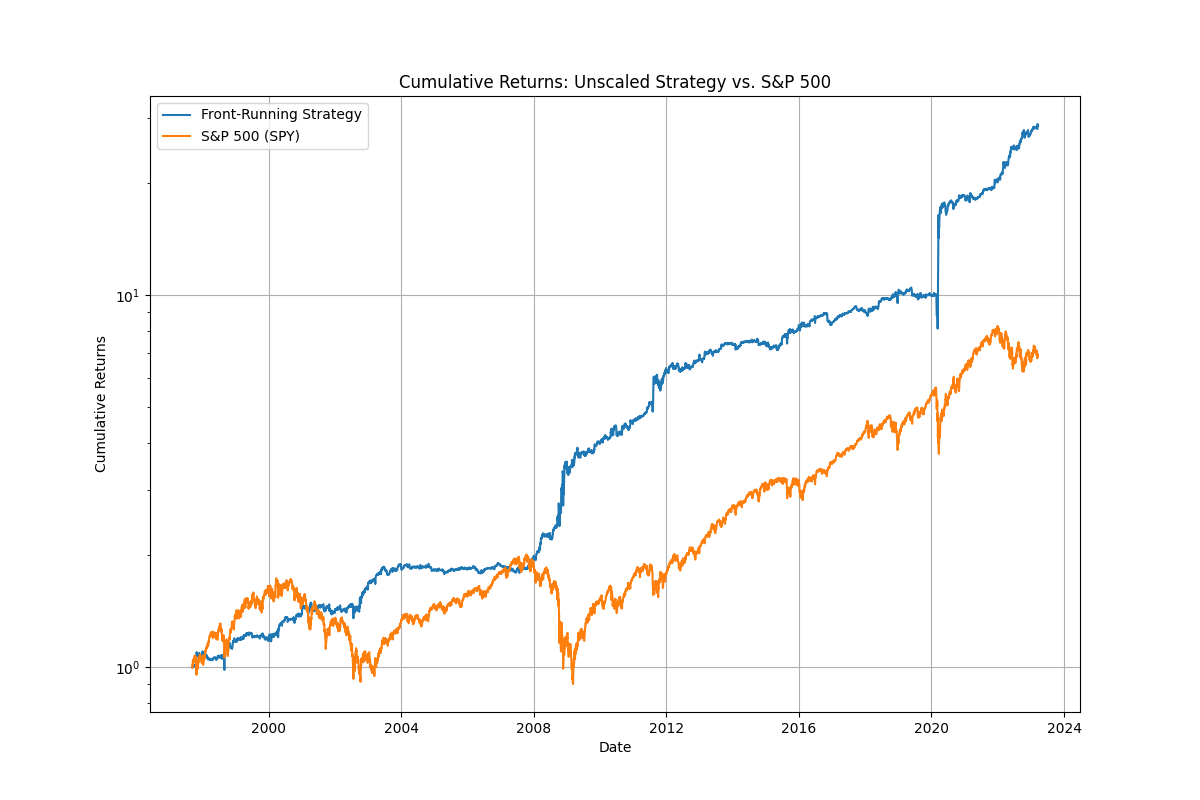
\includegraphics[width=0.8\textwidth]{performance.png}
\caption{Baseline Performance (1997--2023, Log Scale)}
\end{figure}

The performance is strong, with a high Sharpe ratio and lower drawdown than the benchmark. However, this performance hides issues related to turnover.

\subsection{Visualizing the Unfiltered Strategy's Behavior}
To understand the strategy's characteristics, we visualize its relationship with the market over time. Figure~\ref{fig:rolling_metrics} plots the 1-year rolling alpha and beta of the original, unfiltered strategy.

\begin{figure}[htbp]
    \centering
    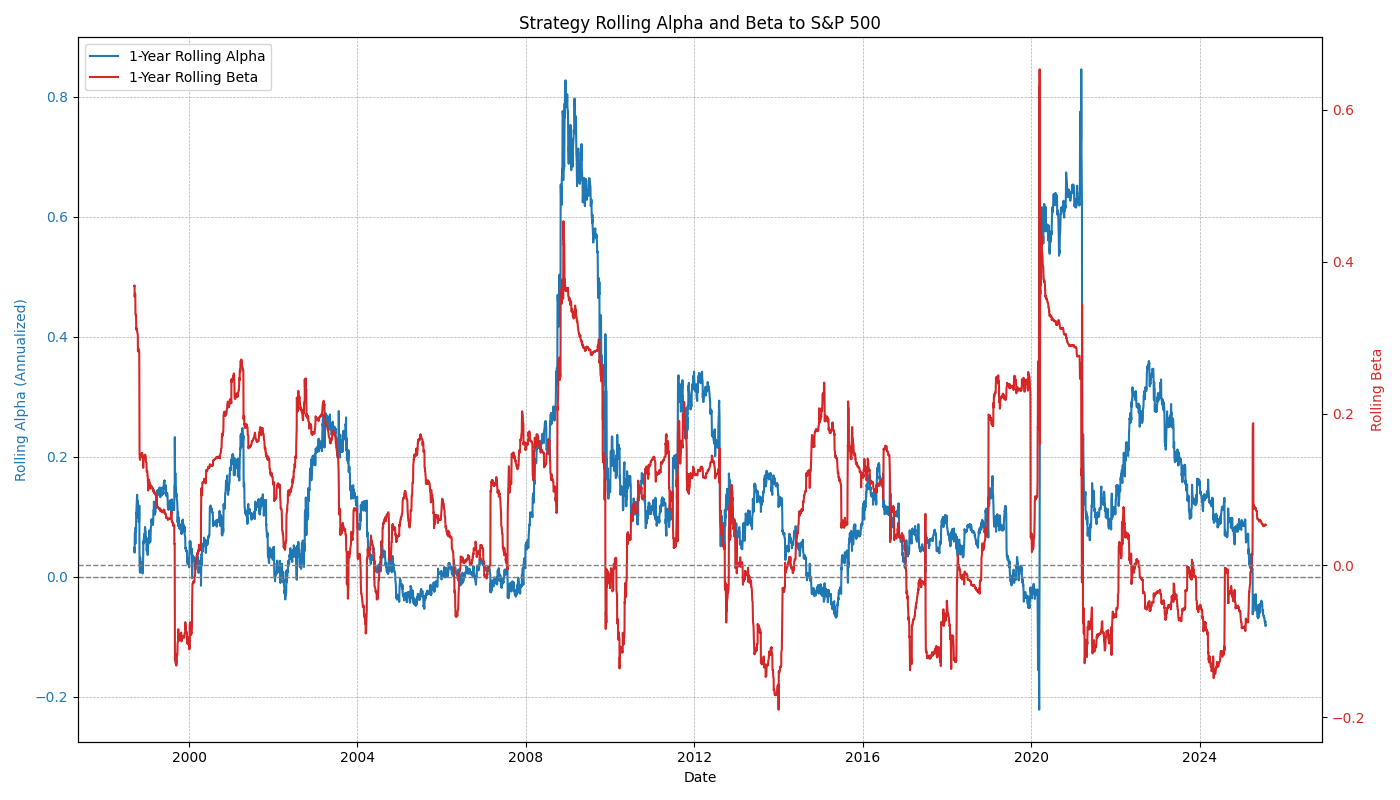
\includegraphics[width=0.8\textwidth]{plot_rolling_metrics.png}
    \caption{Rolling Alpha and Beta of the Unfiltered Dual-Signal Strategy}
    \label{fig:rolling_metrics}
\end{figure}

The plot illustrates the strategy's dual nature. The rolling beta hovers near zero for long periods, indicating no correlation to the S\&P 500. However, during market crises (e.g., 2002, 2008, 2020), the beta often turns negative, confirming its hedging properties. Correspondingly, the annualized alpha increases during these same periods, demonstrating that the strategy's outperformance is not steady but delivered in short bursts. This visualization confirms that the original strategy is fundamentally a crisis-hedging strategy.

\subsection{The Turnover Problem}
The strategy's primary weakness is its high turnover. A detailed analysis reveals how each refinement of the strategy addresses this issue.

\begin{table}[htbp]
\centering
\caption{Annualized Turnover by Strategy Version}
\begin{tabular}{lr}
\toprule
\textbf{Strategy Version} & \textbf{Annualized Turnover} \\
\midrule
Original Dual-Signal      & 54.90 \\
Retail (Calendar-Only)    & 41.96 \\
Final Hedged Equity       & 5.18  \\
\bottomrule
\end{tabular}
\end{table}

An annual turnover of nearly 55 for the original strategy is high for most investors. The table below quantifies the impact of transaction costs on the original dual-signal strategy's performance.

\begin{table}[htbp]
\centering
\caption{Original Strategy Performance vs. Transaction Costs}
\begin{tabular}{lrr}
\toprule
\textbf{Cost (bps per trade)} & \textbf{Strategy CAGR} & \textbf{Strategy Sharpe} \\
\midrule
0          & 14.09\%        & 0.96            \\
1          & 13.46\%        & 0.92            \\
2          & 12.83\%        & 0.87            \\
5          & 10.98\%        & 0.75            \\
10         & 7.96\%         & 0.55            \\
\bottomrule
\end{tabular}
\end{table}

At 10 bps, the strategy's CAGR is nearly halved and its Sharpe ratio decreases significantly, rendering it non-viable. The daily-adjusting \texttt{Threshold} signal is the primary contributor, with an unweighted annualized turnover of over 70. Removing it in the Retail-Adapted version helps, but the turnover remains high. Only by introducing the VIX filter, which keeps the strategy static for long periods, is the turnover reduced to a practical level.

\begin{figure}[htbp]
    \centering
    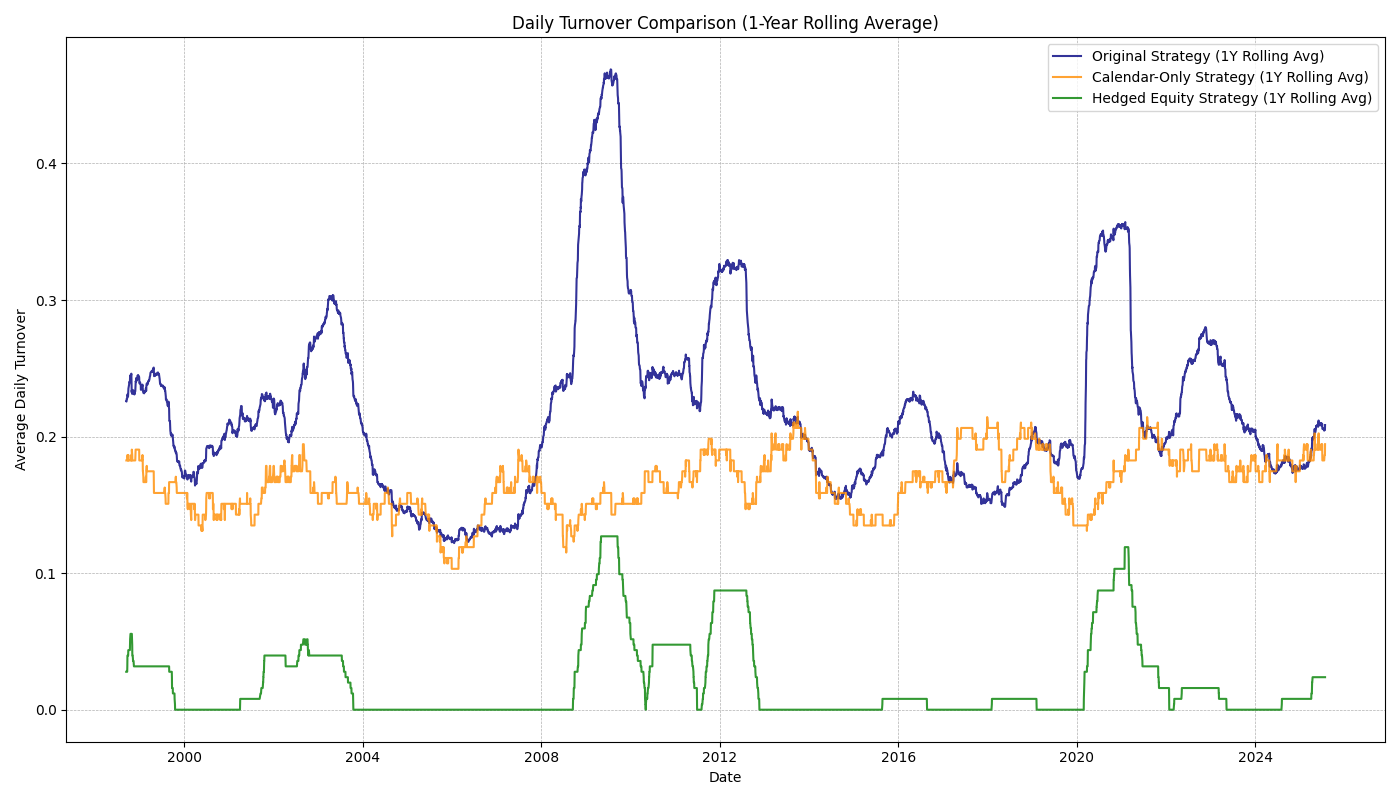
\includegraphics[width=0.8\textwidth]{plot_turnover_analysis.png}
    \caption{Turnover Comparison of Strategy Variations (1-Year Rolling Average)}
    \label{fig:turnover_analysis}
\end{figure}

Figure~\ref{fig:turnover_analysis} visualizes this, showing the reduction in trading frequency achieved by the final Hedged Equity strategy. This reduction is the source of the performance trade-offs discussed next.

\vspace{1em}
\hrulefill

\section{Analysis of Strategy Performance}

\subsection{The ``Crisis Alpha'' Nature of the Anomaly}
Further analysis reveals the strategy's nature. Its performance was analyzed in different market regimes, defined by the VIX index. A reading above 25 indicates a high-volatility period, but not all bear markets are high-VIX events.

\begin{table}[htbp]
\centering
\caption{Performance Comparison in Major Bear Markets}
\begin{tabular}{lrr}
\toprule
\textbf{Metric (Dot-Com Bust)} & \textbf{Hedged Equity} & \textbf{S\&P 500} \\
\midrule
CAGR           & -17.13\% & -22.81\% \\
Max Drawdown   & -39.00\% & -47.41\% \\
\midrule
\textbf{Metric (Global Financial Crisis)} & \textbf{Hedged Equity} & \textbf{S\&P 500} \\
\midrule
CAGR           & -0.71\% & -43.90\% \\
Max Drawdown   & -32.31\% & -55.56\% \\
\bottomrule
\end{tabular}
\end{table}

Our analysis of historical VIX data shows that the dot-com bust was a prolonged bear market that, for the most part, did \textbf{not} trigger the VIX > 20 threshold. Consequently, the Hedged Equity strategy remained largely invested in the S\&P 500, tracking its losses. In contrast, the 2008 Global Financial Crisis was a high-volatility event that kept the hedge active for a sustained period, leading to capital preservation.

This finding is important: the rebalancing anomaly, when filtered by VIX, is a hedge against \textbf{market panic}, not necessarily against bear markets in general.

\begin{figure}[htbp]
\centering
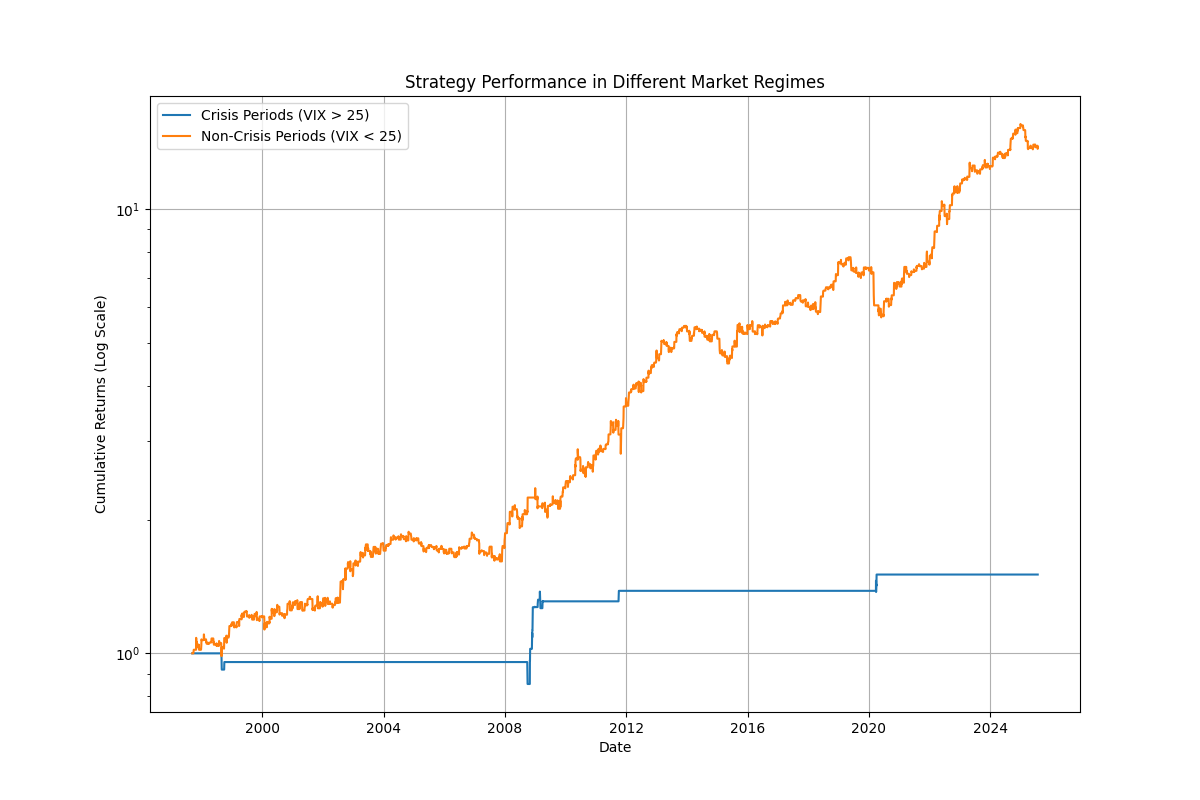
\includegraphics[width=0.8\textwidth]{plot_crisis_analysis.png}
\caption{Strategy Performance in Different Market Regimes}
\end{figure}

\subsection{Walk-Forward Validation: A Test of Robustness}
To address potential overfitting, we employ a \textbf{walk-forward analysis}, which serves as a test of the strategy's \textbf{parameter stability and robustness} across different market regimes.

\begin{figure}[htbp]
\centering
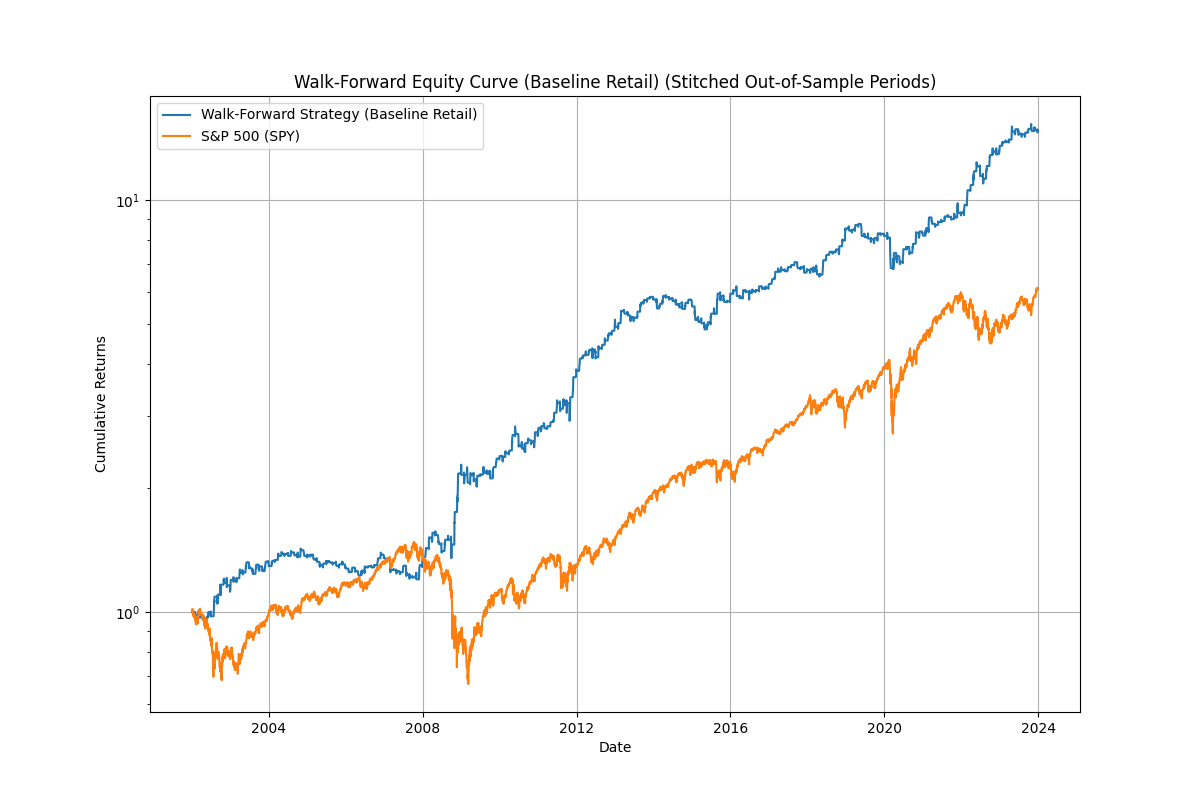
\includegraphics[width=0.8\textwidth]{plot_walk_forward.png}
\caption{Walk-Forward Equity Curve (Baseline Retail Strategy)}
\label{fig:walk_forward}
\end{figure}

The performance in this test (Figure~\ref{fig:walk_forward}) suggests that the strategy's edge is a persistent anomaly. This provides higher confidence in its viability.

\section{The Hedged Equity Strategy}
Our research leads to a final conclusion. A pure hedging strategy creates an opportunity cost by being flat during calm markets. The proposed strategy combines market exposure during calm periods with a protective hedge when markets are stressed.

This \textbf{Hedged Equity Strategy} is defined as follows:
\begin{itemize}
    \item When the VIX is \textbf{below} a set threshold (e.g., 20), the strategy's return is simply the daily return of the S\&P 500 (SPY).
    \item When the VIX is \textbf{above} the threshold, the strategy's return switches to the Calendar-Only hedge (long/short SPY vs. TLT).
\end{itemize}

This approach addresses the low-CAGR issue of a pure hedge while retaining its downside protection. It is an improvement over VIX-filtered models that default to holding cash, as it reduces the opportunity cost of being out of the market.

\subsection{Performance of the Hedged Equity Strategy}
The results of this refined approach are specific. The Hedged Equity strategy essentially matches the long-term return of the S\&P 500 with slightly lower volatility. Its primary value is a reduction in tail risk during specific, high-volatility periods. This benefit is almost entirely concentrated in a few key events, such as the 2008 Global Financial Crisis. In most other periods, including the dot-com bust, the strategy provides no significant alpha and tracks the market.

\begin{table}[htbp]
\centering
\caption{Hedged Equity Strategy Performance (VIX > 20)}
\begin{tabular}{lrr}
\toprule
\textbf{Metric} & \textbf{Hedged Equity} & \textbf{S\&P 500 (SPY)} \\
\midrule
CAGR           & 9.32\%    & 9.26\%         \\
Volatility     & 17.49\%   & 19.61\%        \\
Sharpe Ratio   & 0.53      & 0.47           \\
Max Drawdown   & $-42.54$\% & $-55.14$\%      \\
\bottomrule
\end{tabular}
\end{table}

The value of this strategy is illustrated visually. Figure~\ref{fig:hedged_equity_curve} shows the strategy's cumulative returns against the S\&P 500. It tracks the market closely during calm periods but diverges during major events like the 2008 GFC and the 2020 COVID-19 crash. Figure~\ref{fig:hedged_equity_drawdowns} shows that while the S\&P 500's drawdown exceeded 55\%, the Hedged Equity strategy's was contained to 42.5\%.

\begin{figure}[htbp]
    \centering
    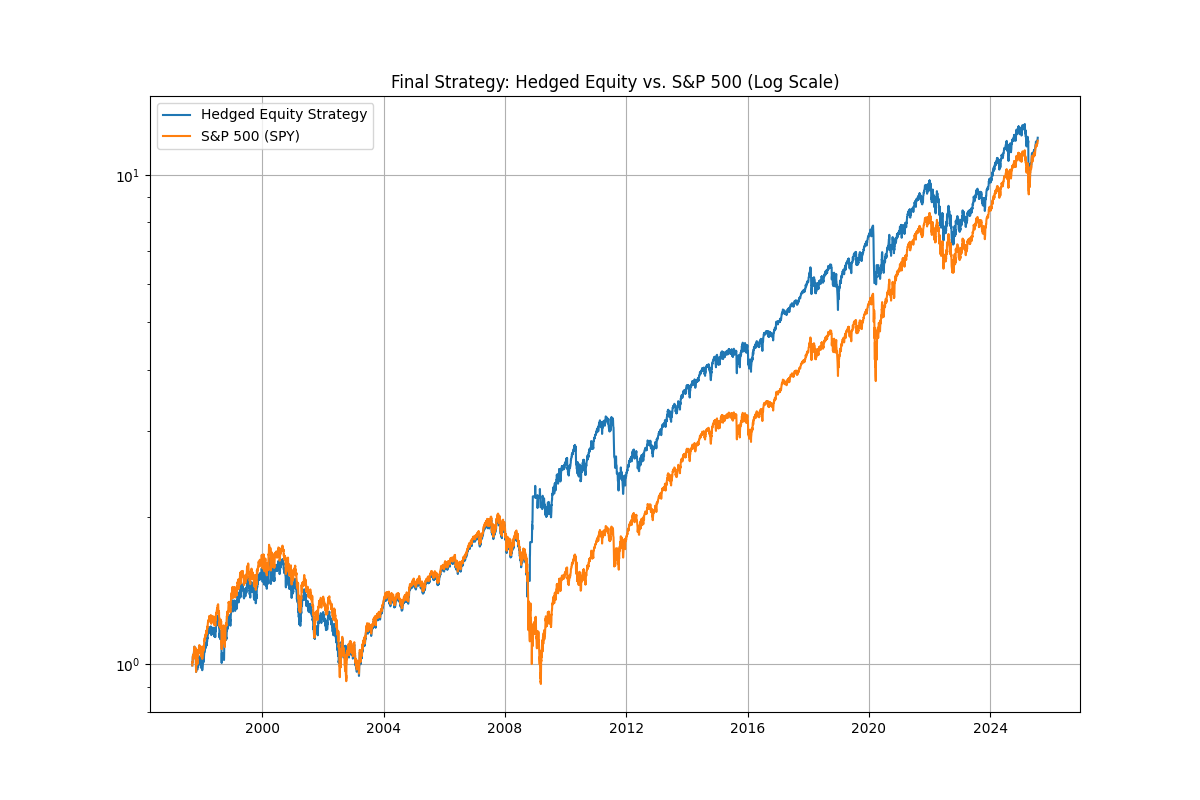
\includegraphics[width=0.8\textwidth]{plot_hedged_equity_curve.png}
    \caption{Final Strategy: Hedged Equity vs. S\&P 500}
    \label{fig:hedged_equity_curve}
\end{figure}

\begin{figure}[htbp]
    \centering
    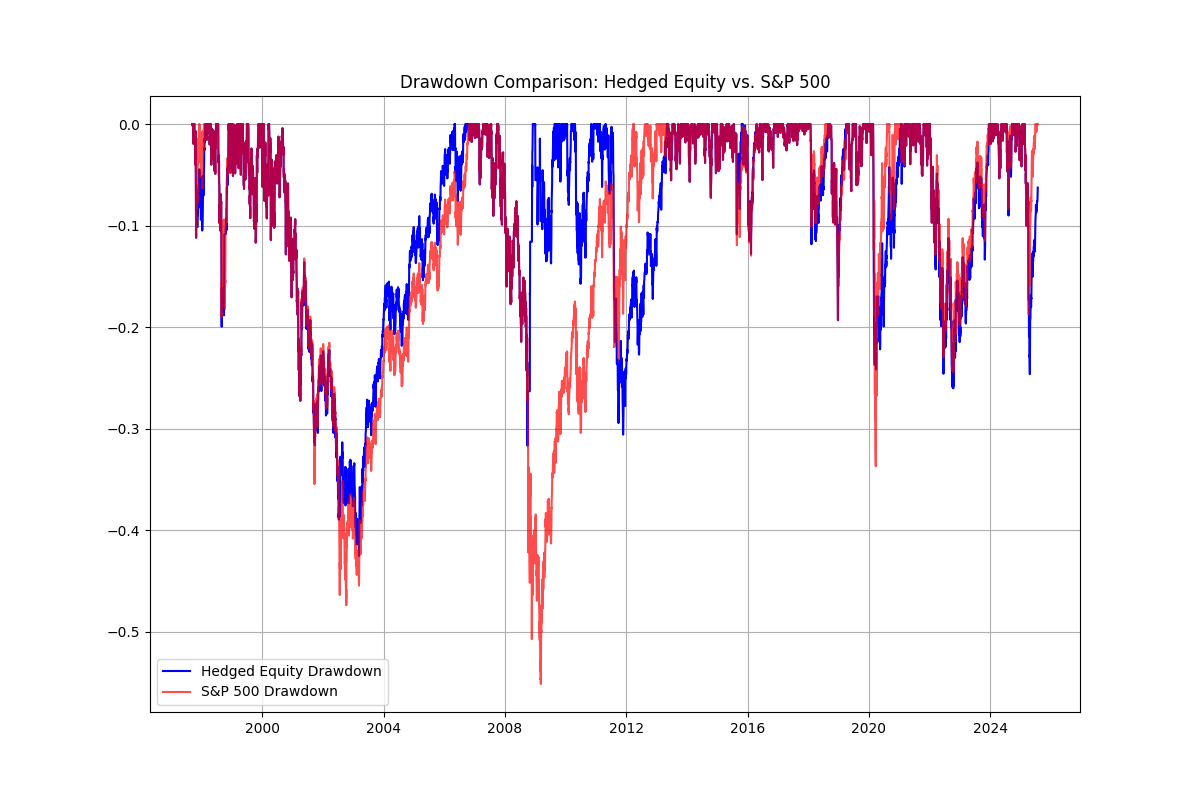
\includegraphics[width=0.8\textwidth]{plot_hedged_equity_drawdowns.png}
    \caption{Final Strategy: Drawdown Comparison}
    \label{fig:hedged_equity_drawdowns}
\end{figure}

\subsection{Walk-Forward Validation of the Hedged Equity Strategy}
To test the robustness of this refined strategy, we performed a walk-forward analysis. This provides a test of its viability by simulating how it would have performed on unseen data over time.

\begin{table}[htbp]
\centering
\caption{Hedged Equity Walk-Forward Performance (VIX > 20)}
\begin{tabular}{lrr}
\toprule
\textbf{Metric} & \textbf{Strategy} & \textbf{S\&P 500 (SPY)} \\
\midrule
CAGR           & 9.63\%    & 8.61\%         \\
Sharpe Ratio   & 0.57      & 0.45           \\
Max Drawdown   & $-31.07$\% & $-54.75$\%      \\
Annual Turnover & 5.20      & ---            \\
\bottomrule
\end{tabular}
\end{table}

The out-of-sample results confirm the strategy's specific nature. While the risk-adjusted returns remain positive, the strategy's value is dependent on the presence of infrequent, high-VIX events in the test window. The reduction in drawdown is notable but should not be misinterpreted as a general-purpose bear market hedge. The results suggest the mechanism is not random, but its applicability is limited.

\begin{figure}[htbp]
\centering
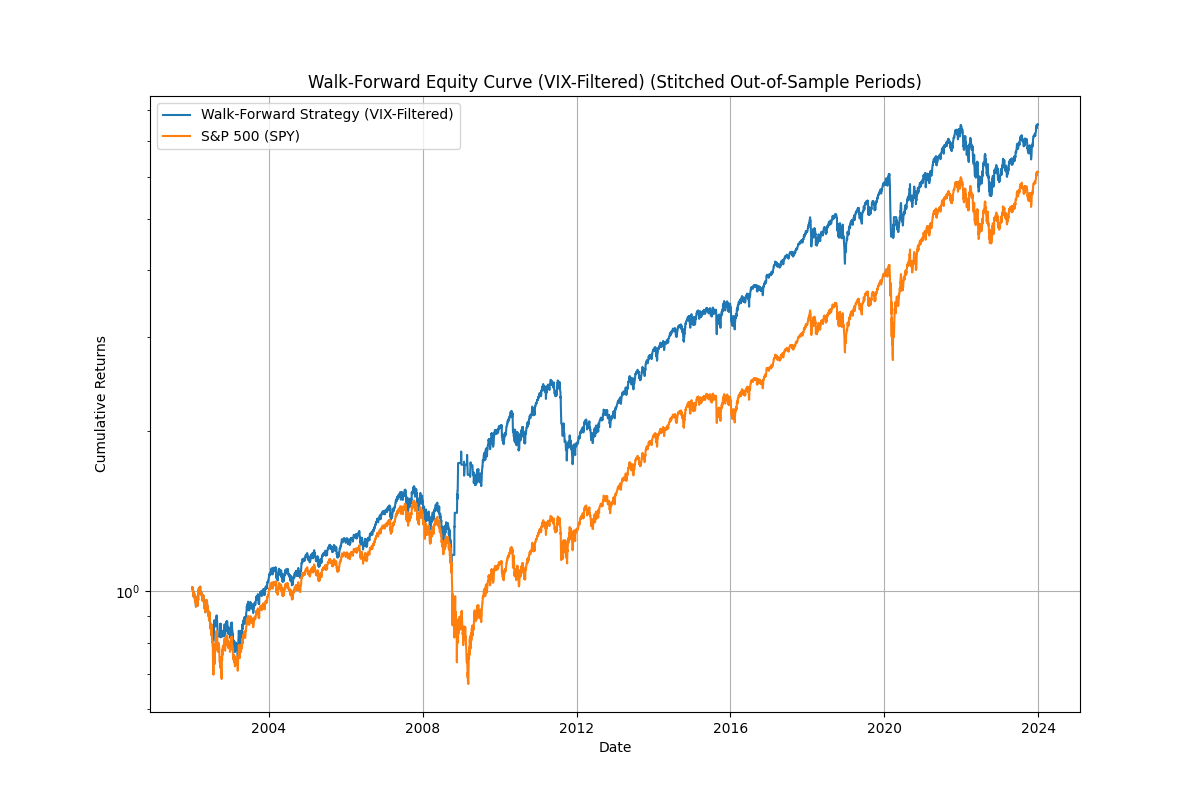
\includegraphics[width=0.8\textwidth]{plot_walk_forward_vix_filtered.png}
\caption{Hedged Equity Walk-Forward Equity Curve}
\label{fig:walk_forward_vix}
\end{figure}

\subsection{A Variation: The 200-Day Moving Average Filter}
\label{sec:ma_filter}
As a variation on the VIX-filtered approach, we explored using a simple 200-day moving average (MA) of the S\&P 500 as an alternative trigger for the hedge. The logic is that the hedge is most valuable during sustained downturns, which a 200-day MA is well-suited to identify.

The strategy is defined as follows:
\begin{itemize}
    \item When the S\&P 500 is \textbf{above} its 200-day MA, the strategy's return is the daily return of the S\&P 500 (SPY).
    \item When the S\&P 500 is \textbf{below} its 200-day MA, the strategy's return switches to the Calendar-Only hedge.
\end{itemize}

\begin{table}[htbp]
\centering
\caption{Hedged Equity Strategy Performance (200-Day MA Filter)}
\begin{tabular}{lrr}
\toprule
\textbf{Metric} & \textbf{MA-Filtered Strategy} & \textbf{S\&P 500 (SPY)} \\
\midrule
CAGR           & 12.60\%    & 7.14\%         \\
Volatility     & 15.73\%   & 19.94\%        \\
Sharpe Ratio   & 0.80      & 0.36           \\
Max Drawdown   & -26.77\% & -55.14\%      \\
\bottomrule
\end{tabular}
\end{table}

\begin{figure}[htbp]
    \centering
    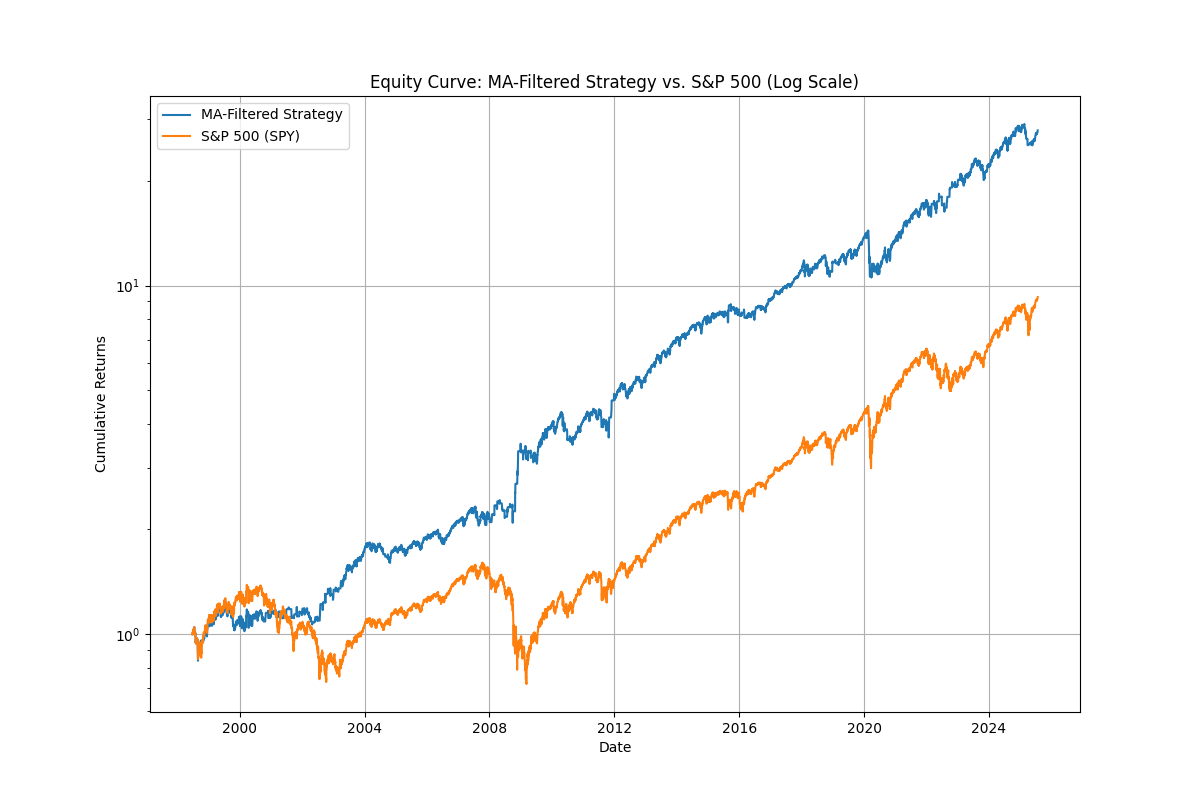
\includegraphics[width=0.8\textwidth]{plot_ma_strategy_equity_curve.png}
    \caption{MA-Filtered Strategy vs. S\&P 500}
    \label{fig:ma_filtered_equity_curve}
\end{figure}

\begin{figure}[htbp]
    \centering
    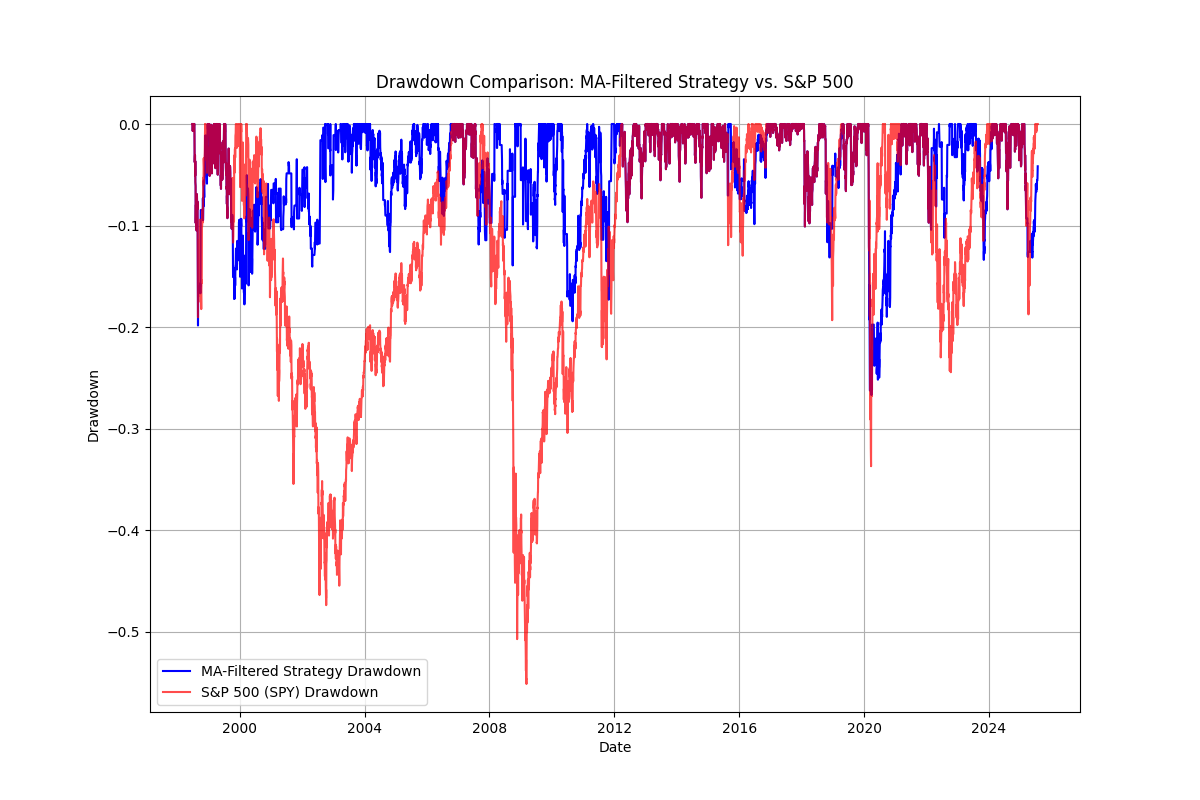
\includegraphics[width=0.8\textwidth]{plot_ma_strategy_drawdowns.png}
    \caption{MA-Filtered Strategy: Drawdown Comparison}
    \label{fig:ma_filtered_drawdowns}
\end{figure}

The results of this variation are compelling. The MA-filtered strategy outperforms both the S\&P 500 and the VIX-filtered strategy on a risk-adjusted basis, with a higher Sharpe ratio and a lower maximum drawdown. This suggests that the 200-day moving average is a more effective filter for activating the hedge, as it is less prone to the short-term spikes that can affect the VIX.

\subsection{Monte Carlo Simulation: Understanding the Risk}
\label{sec:monte_carlo}
A strategy can have long periods of underperformance. To understand the range of potential outcomes and the importance of a long investment horizon, we use a \textbf{Monte Carlo simulation}. This technique involves creating thousands of possible future return paths by randomly sampling from the strategy's historical daily returns.

\begin{table}[htbp]
\centering
\caption{Probability of Underperformance vs. Horizon}
\begin{tabular}{lrr}
\toprule
\textbf{Horizon} & \textbf{Prob. of Loss} & \textbf{Prob. Underperform SPY} \\
\midrule
1 Year  & 18.84\%        & 46.62\%                 \\
3 Years & 7.24\%         & 43.24\%                 \\
5 Years & 2.94\%         & 43.74\%                 \\
10 Years & 0.58\%         & 38.12\%                 \\
20 Years & 0.00\%         & 35.32\%                 \\
\bottomrule
\end{tabular}
\end{table}

\begin{figure}[htbp]
\centering
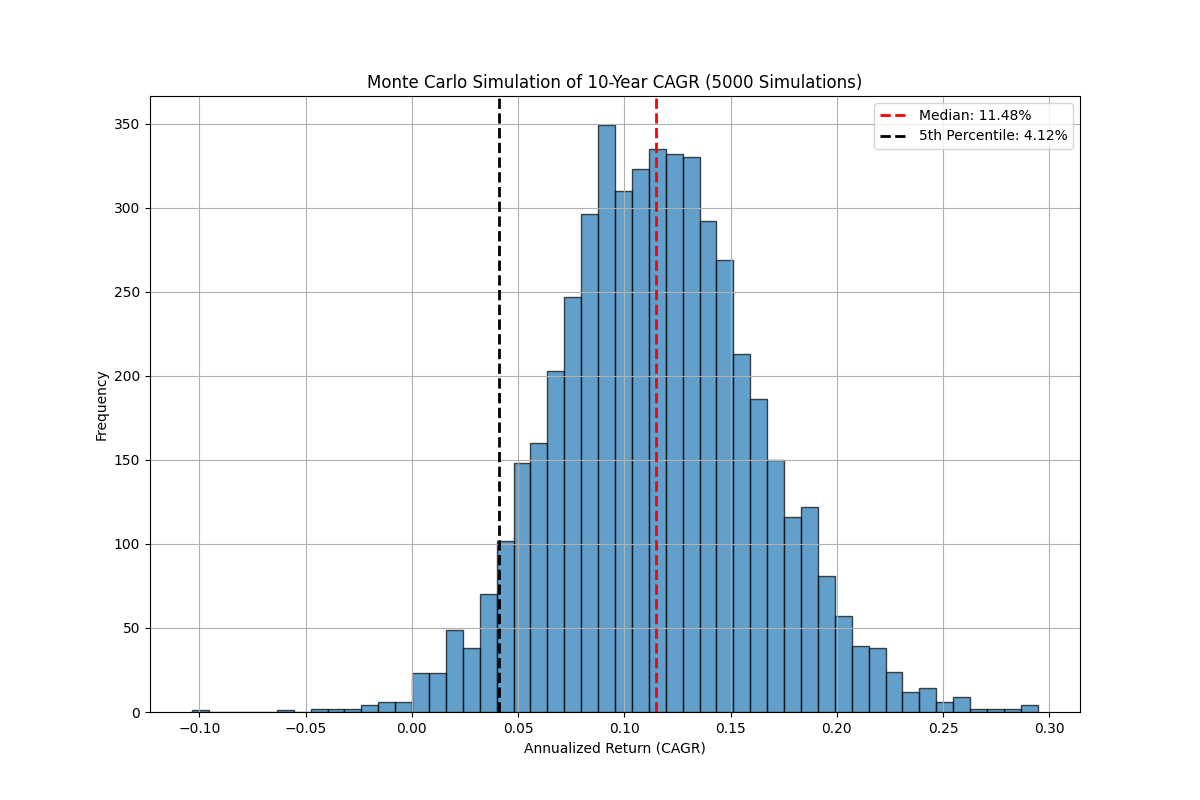
\includegraphics[width=0.8\textwidth]{plot_monte_carlo.png}
\caption{Monte Carlo CAGR Distribution (10-Year Horizon)}
\end{figure}

The simulation provides a useful perspective. Over a 1-year horizon, there is a 47\% chance of underperforming the market. The probability of loss is also non-trivial. Only by extending the investment horizon to \textbf{5--10 years} is the probability of a negative outcome reduced and the probability of outperformance becomes higher. This analysis suggests that capturing the benefits of this strategy requires a long-term commitment.

\vspace{1em}
\hrulefill

\section{Conclusion}
The ``rebalancing anomaly'' is a historically persistent phenomenon, but its practical application has challenges. The original dual-signal model is non-viable due to high turnover.

Our refinement leads to the \textbf{Hedged Equity Strategy}, but its benefits are specific. The strategy is best understood as a low-turnover method for capturing market beta with a built-in, specific hedge against volatility panics. Most of its historical alpha was generated during the 2008 crisis. Outside of such infrequent events, it offers little advantage over simply holding the S\&P 500, and does not protect against prolonged bear markets like the dot-com bust.

The conclusion is that the Hedged Equity strategy is not a source of consistent alpha but a tool for tail-risk hedging. Its value is dependent on the occurrence of infrequent, panic-driven events. An investor must accept long periods of market-tracking performance for the potential of mitigation during these events. It is a tool for a long-term investor who understands these limitations.

\end{document}